\subsection*{Background}

\subsubsection*{GAN}

Generative Adversarial Networks trains a generator $G$ and a discriminator $D$ together though a mini-max game
The generator takes in random noise and maps the noise to an image.
The discriminator takes in an image and tells if it is real from the dataset or generated by the generator.
To train these two network simultaneously, Goodfellow et al. defined the loss function as 
$$
\min_G\max_{D}\mathcal{L}(D, G) = 
\mathbb{E}_{x \sim p_{data}}[\log D(x)] + 
\mathbb{E}_{z \sim p_z}[\log (1 - D(G(z)))]
$$
where $p_{data}$ is the images in the real dataset
and $p_z$ is randomly generated vectors in the same shape as the real images \cite{Goodfellow2020Generative}.

\par
Based on the above models, Karras et al. proposed StyleGAN as 
a GAN variant that can separate high-level feature variations and scale-specific control these variations \cite{Karras2019Style}.
If trained on a dataset of human faces, these high-level features including eyes, nose, hair, etc.
Together with GAN's two model nature, mapping the high-level features of anime characters to real human pictures becomes possible.
Min Jin Chong and Davis Forsyth proposed two GAN-based models,
GANs N' Roses (GNR) and JoJoGAN,
to map anime image style to human pictures \cite{chong2021gans,chong2021jojogan}.
GNR trained on different anime characters will learn different styles,
thus produces a sequence of diverse outputs based on the same input image.
\begin{figure}[h]
    \includegraphics[width=\textwidth]{img/GNR-1.png}
    \caption{
        GANs N' Roses: The first column on the left is the input human picture.
        Each following column shows a different style learned from different anime mapped to that human \cite{chong2021gans}.
    }
\end{figure}

JoJoGAN, however, takes in an anime character's image as reference and generates
a style mapper that can be applied to human faces.
The key difference between JoJoGAN and GNR is that GNR needs a dataset of same anime character to learn the style of that character.
Instead of finding a large amount of quality images of same character,
JoJoGAN can be trained on a generalized anime dataset,
then produce the need style map based on the given single reference.
This difference allows JoJoGAN to generate multiple images of multiple much easier than other style-based image generator.
\begin{figure}[h]
    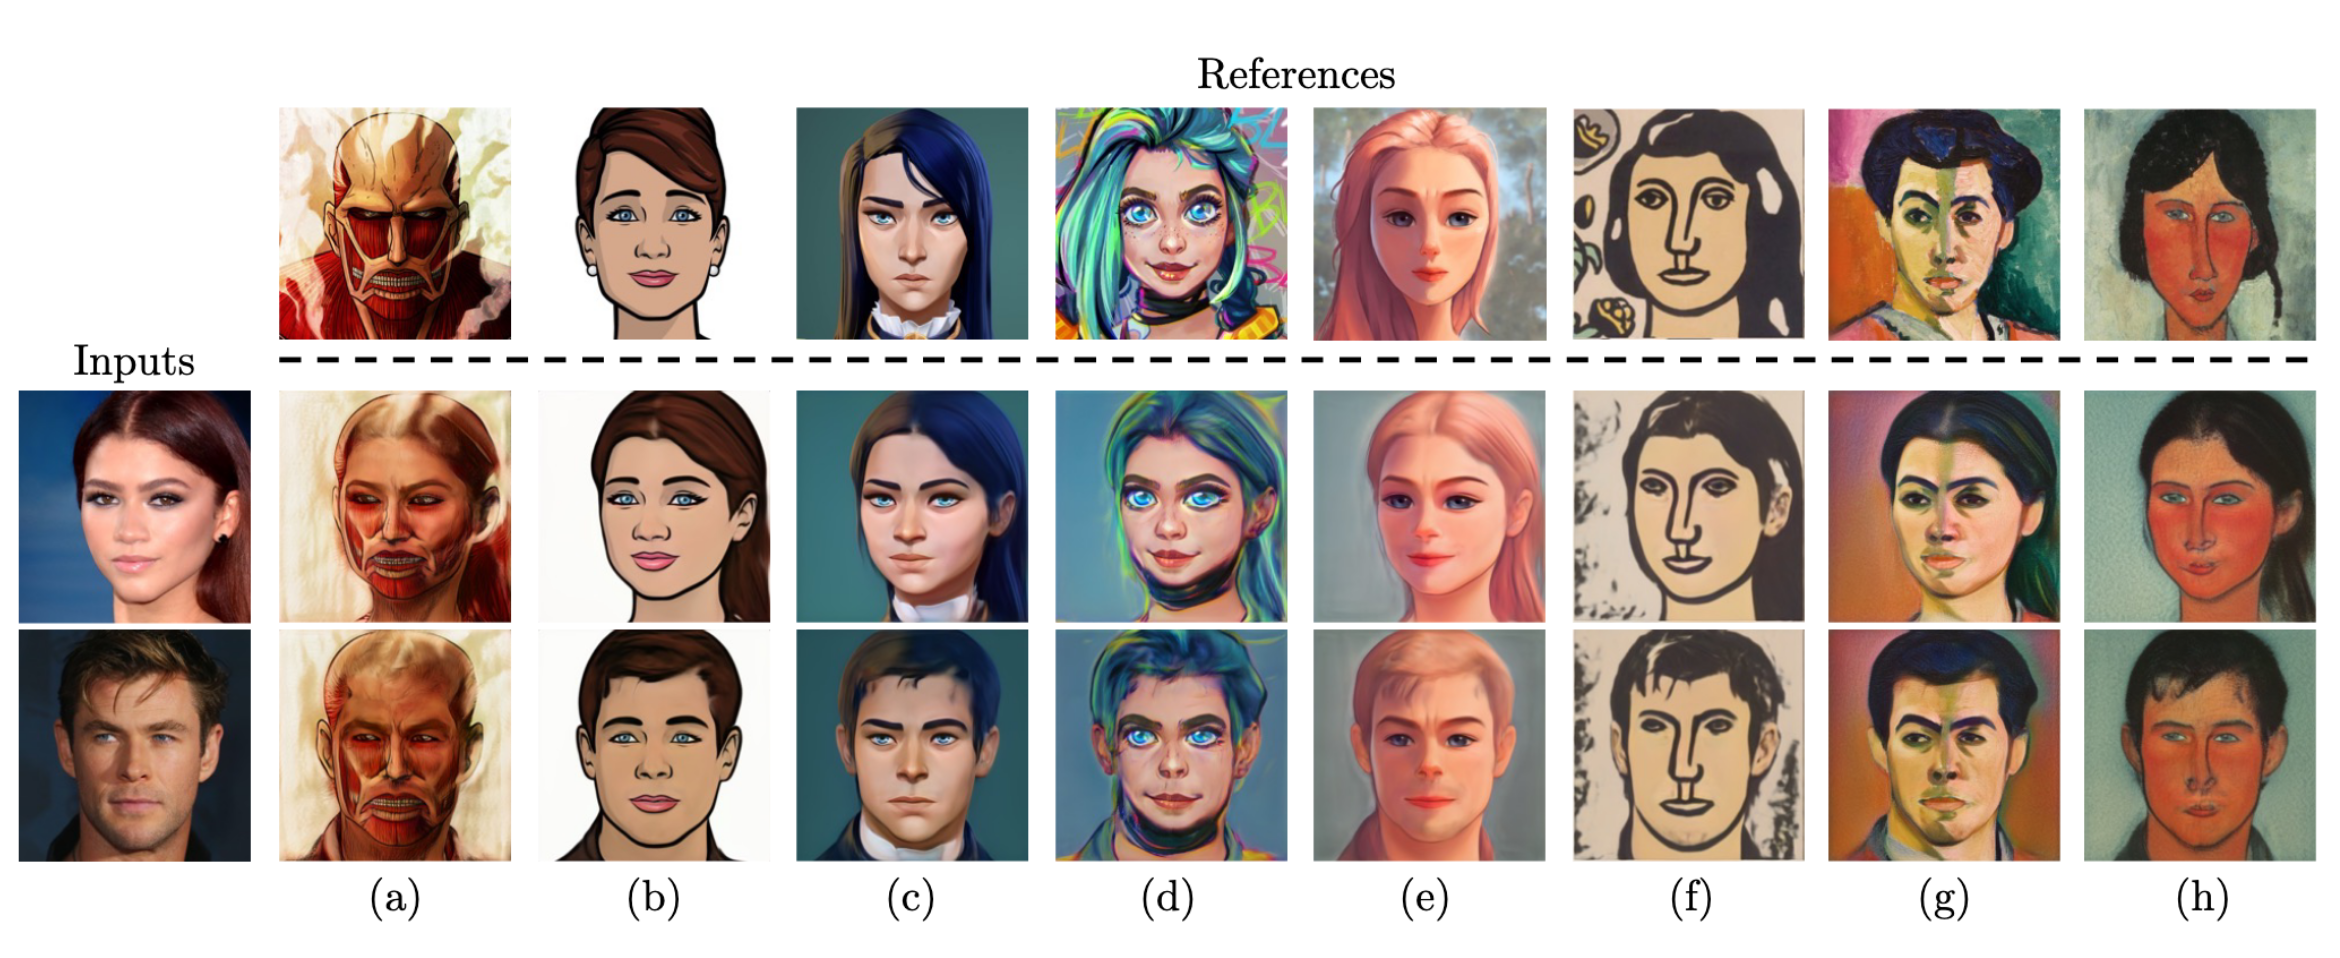
\includegraphics[width=\textwidth]{img/JoJo-1.png}
    \caption{
        JoJoGAN: The first column on the left is the input human picture.
        Each following column shows a different style generated from different reference anime image \cite{chong2021jojogan}.
    }
\end{figure}

\subsubsection*{Diffusion Models}

Rombach et al. newly proposed Latent Diffusion Models as the state-of-art image generation algorithm \cite{Rombach2022High}.
The idea of diffusion is to learn an image style by denoising the training image to learn the data distribution in the image.
That is, gradually break down am image into noises.
Then for generation, they use the inverse map of diffusion to resample on noise under known distribution

$$
L_{L D M}:=\mathbb{E}_{\mathcal{E}(x), \epsilon \sim \mathcal{N}(0,1), t}\left[\left\|\epsilon-\epsilon_\theta\left(z_t, t\right)\right\|_2^2\right]
$$

As StyleGAN models specialized on image-to-image generation,
LDMs shows surprising results on text-to-image generation as shown in Figure 3.
\begin{figure}[]
    \includegraphics[width=\textwidth]{img/LDM-1.png}
    \caption{
        Latent Diffusion Models:
        user input text are on the top
        and the generated images are under the text descriptions \cite{Rombach2022High}.
    }
\end{figure}

When we apply LDM to anime characters,
we can easily generate any character as we want with proper text description as in Figure 4.
As shown in the image grid,
text-to-image generated images are like brand-new characters,
i.e. there is hard to find the exact same style character in existing anime as in StyleGAN generated images.
\begin{figure}[h]
    \begin{center}
    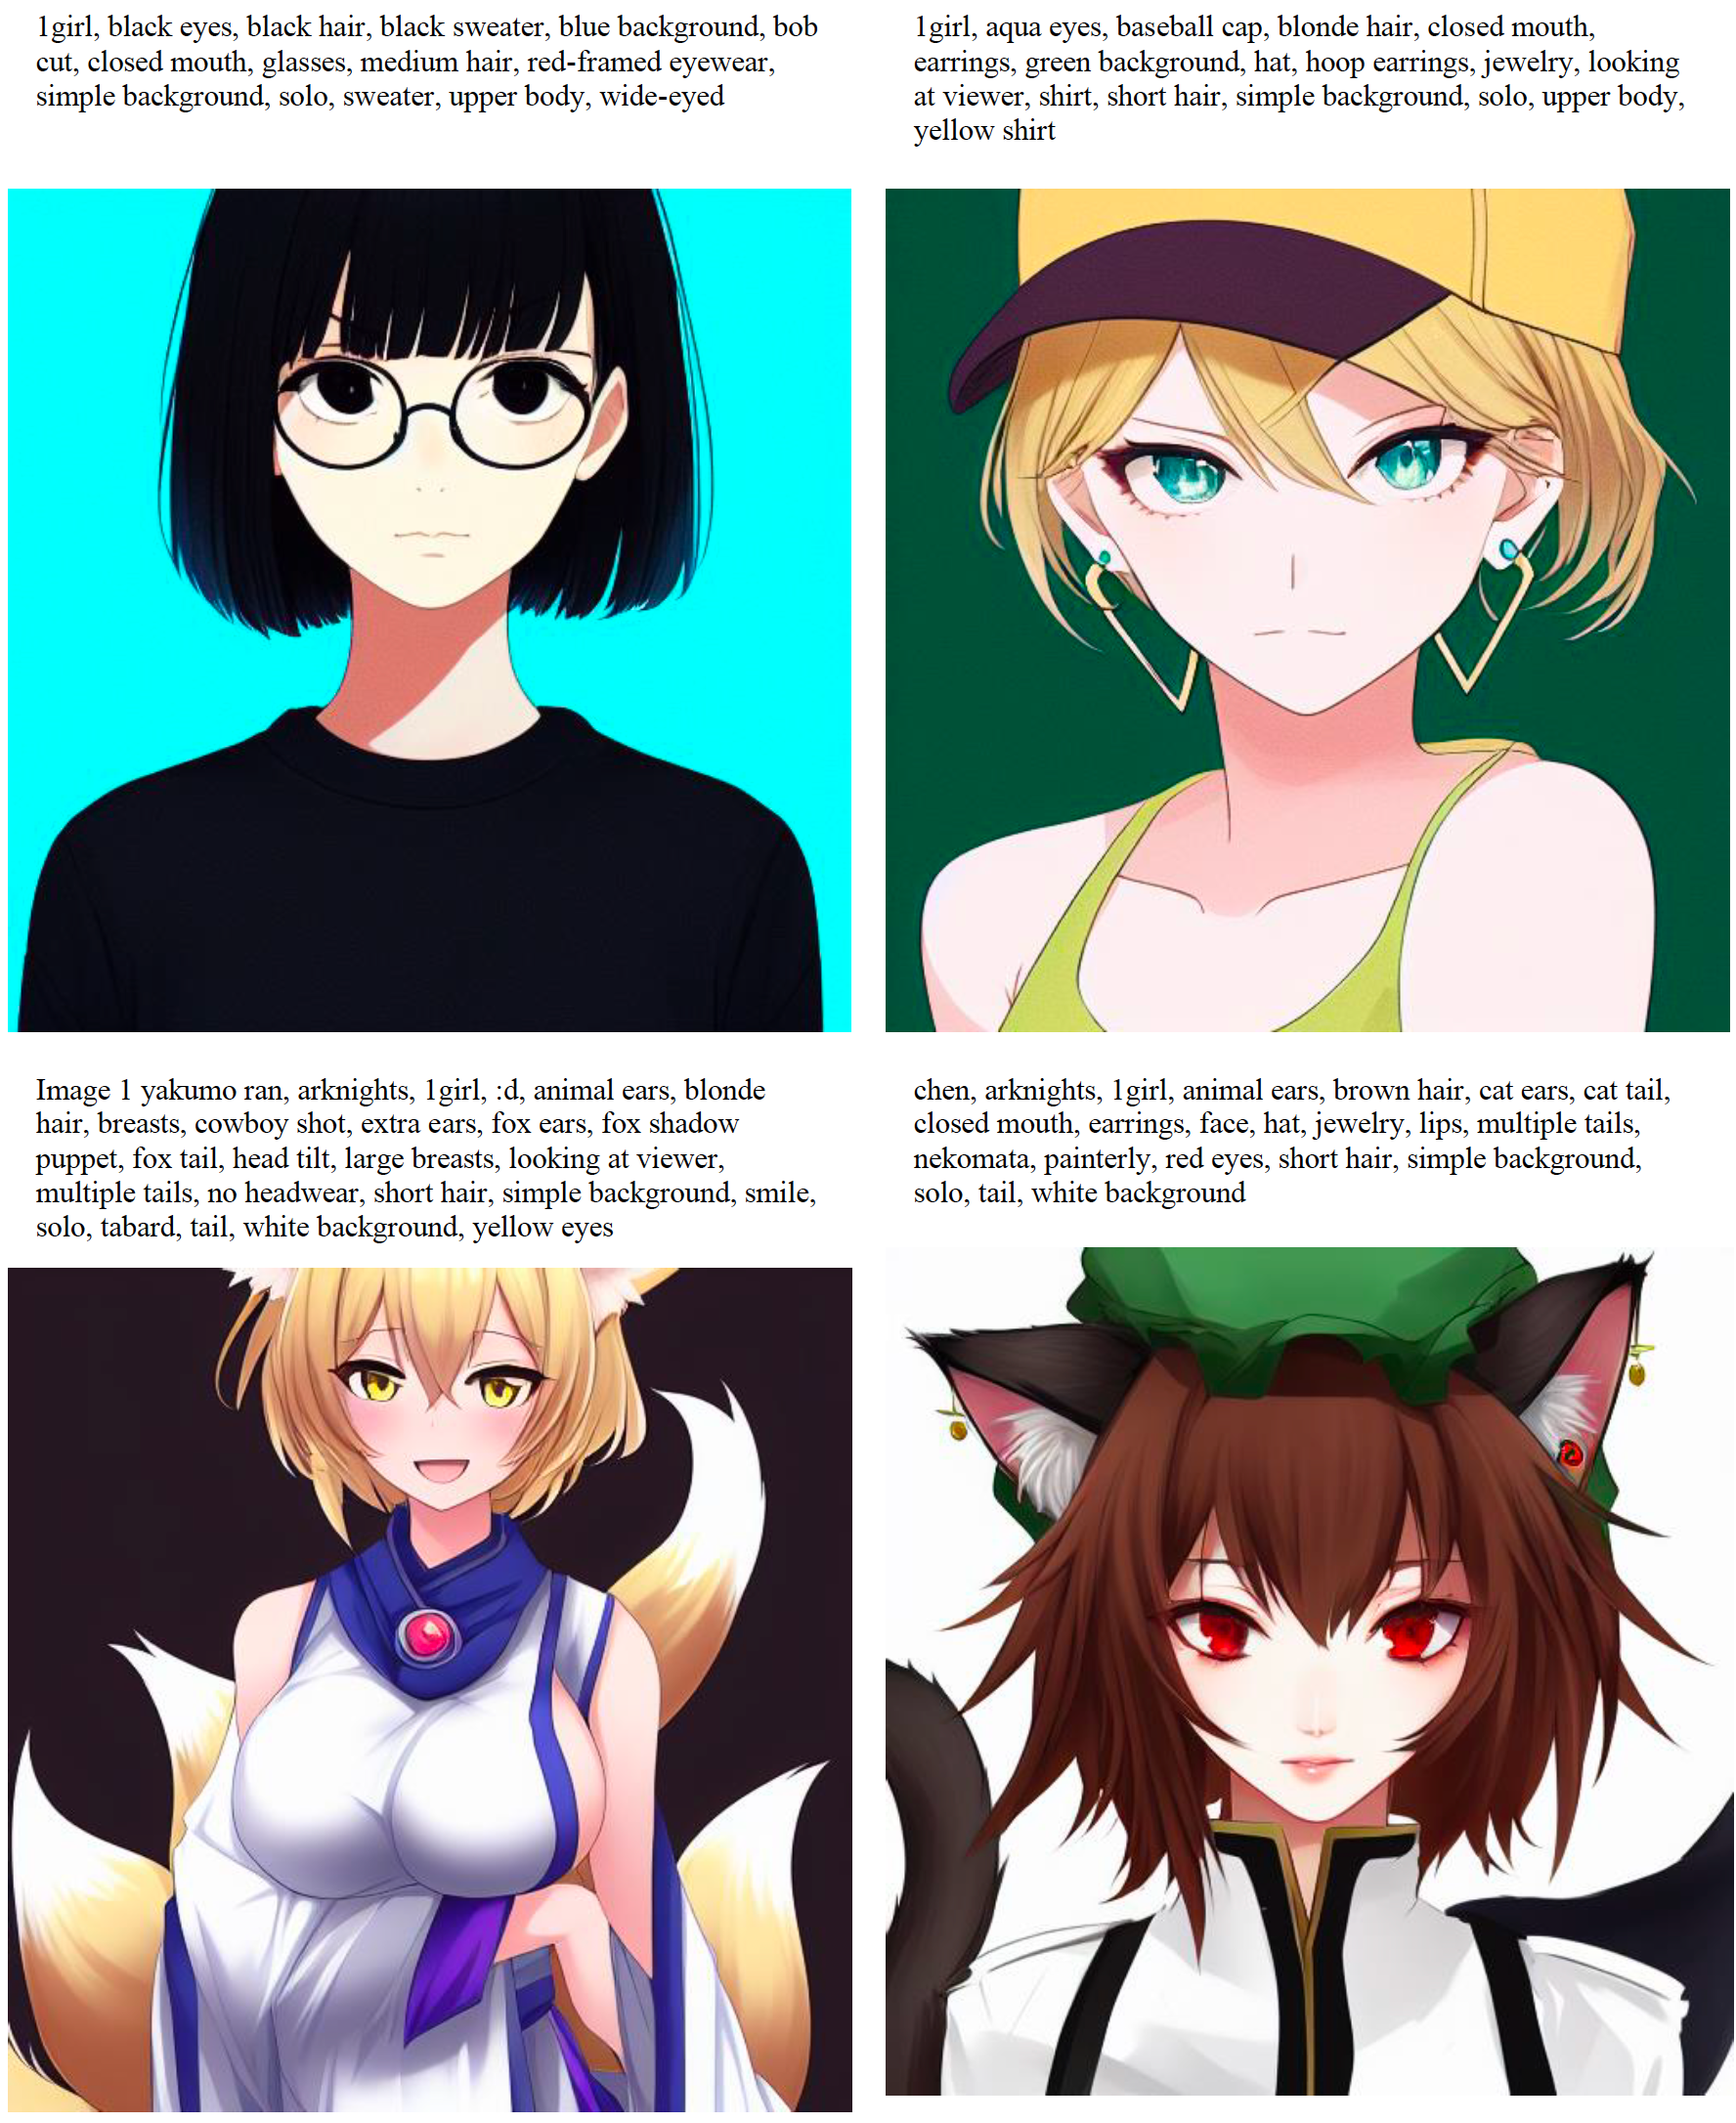
\includegraphics[width=0.78\textwidth]{img/waifu_diffusion.png}
    \end{center}
    \caption{
        Waifu Diffusion:
        user input text are on the top
        and the generated images are under the text descriptions \cite{WaifuDiffusion}.
    }
\end{figure}